\documentclass[11pt]{article}

\usepackage{amsmath}
\usepackage{amssymb}
\usepackage[utf8]{inputenc}
%\usepackage[latin1]{inputenc}
\usepackage[spanish]{babel}
\usepackage[left=3cm,right=3cm,top=3cm,bottom=2.5cm]{geometry}
\usepackage{amsmath,amssymb,latexsym,color,graphicx,verbatim}
\usepackage{mathrsfs}
\usepackage{layout}
\usepackage{graphicx}
\usepackage{multirow}
\usepackage[table,xcdraw]{xcolor}
%COLOCA COMANDOS EN ESPAÑOL
%\renewcommand{\contentsname}{Contenido}
%\renewcommand{\partname}{Parte}
%\renewcommand{\appendixname}{Apéndice}
%\renewcommand{\figurename}{Figura}
%\renewcommand{\tablename}{Tabla}
%\renewcommand{\abstractname}{Resumen}
%\renewcommand{\refname}{Bibliografía}
%FIN DEL BLOQUE
\usepackage[acronym,shortcuts]{glossaries} %PARA UN GLOSARIO DE ACRÓNIMOS
\makeglossaries
\usepackage[font=small]{caption}
\usepackage[colorlinks = true,
                     linkcolor = blue,
                     citecolor = red,
                     urlcolor = blue]{hyperref}

\baselineskip0.75cm
\parskip0.5cm
\parindent0cm

\begin{document}


\begin{titlepage}
\centering {\Large {\sc Estudio del último eclipse cromosférico de Zeta Aurigae, otoño 2019}}

\vfill
\centering {\Large Propuesta de trabajo de grado para optar al t\'itulo de F\'isica}
\vfill
\hfill

\centering {\Large Natalia Lucía Oliveros Gómez$^{1,2}$}

\vfill

\centering {\Large Director: Ph. D Klaus-Peter Schröder $^{3}$}

\centering {\Large  Co-Director: Ph.D Luis Alberto Núñez$^{1,2}$}

\centering {\Large  Co-Director: M. Sc Faiber Danilo Rosas$^{3}$}


\hfill




{{\Large $^1$Grupo de Investigaci\'on en Relatividad y Gravitaci\'on GIRG}} \\
{{\Large$^2$Grupo Halley de Astronom\'ia y Ciencias Aeroespaciales}} \\
{{\Large$^3$Universidad de Guanajuato}} \\

\vfill
\vfill

\centering {\Large Universidad Industrial de Santander\\Facultad de
Ciencias\\Escuela de F\'{i}sica\\Bucaramanga\\2020}


\end{titlepage}


\newpage

\tableofcontents

%\newpage

%\acrodef{LAGO}{Latin American Giant Observatory}

\newpage




%%%%%%%%%%%%%%%%%%%%%%%%%%%%%%%%%%%%%%%%%%%%%%%%%%%%%%%%%%%%%%%%%%%%%%%%%%%%%%%%%%%%%%%%%%%%%%

\begin{table}[htbp]
\begin{center}
\resizebox{14cm}{!}{
\begin{tabular}{|l|l|l|l|l|}
\hline
\multicolumn{5}{|l|}{\begin{tabular}[c]{@{}l@{}}\textbf{Título de la propuesta:}\\ Estudio del último eclipse cromosférico de Zeta Aurigae, otoño 2019\end{tabular}}           \\ \hline
\multicolumn{5}{|l|}{\begin{tabular}[c]{@{}l@{}}\textbf{Nombre del estudiante:}\\ Natalia Lucía Oliveros Gómez\end{tabular}}                                                    \\ \hline
\textbf{Código:} 2160778                          & \multicolumn{3}{l|}{\textbf{E-mail:} onatalialucia@gmail.com}                              & \textbf{Cel:} 3123154756                         \\ \hline
\multicolumn{5}{|l|}{\begin{tabular}[c]{@{}l@{}}\textbf{Nombre del grupo de Investigación:}\\ Universidad de Guanajuato\end{tabular}}                                           \\ \hline
\multicolumn{5}{|l|}{\textbf{Dirrección:} Guanajuato, Guanajuato, México}                                                                                                       \\ \hline
\textbf{Tel:}                                     & \multicolumn{4}{l|}{\textbf{E-mail:}}                                                                                                \\ \hline
\multicolumn{5}{|l|}{\textbf{Líneas de investigación desarrolladas por el grupo:} Física estelar }             \\ \hline
\multicolumn{5}{|l|}{\begin{tabular}[c]{@{}l@{}}\textbf{Profesor de la Escuela de Física que dirigirá el trabajo:}\\ Ph. D Luis Alberto Núñez de Villavicencio Martínez\end{tabular}} \\ \hline
\multicolumn{5}{|l|}{\begin{tabular}[c]{@{}l@{}}\textbf{Profesional del grupo de investigación que servirá de tutor:}\\ Ph. D Klaus-Peter Shrörder\end{tabular}}                      \\ \hline
\end{tabular}}
\end{center}
\end{table}

\newpage
%%%%%%%%%%%%%%%%%%%%%%%%%%%%%%%%%%%%%%%%%%%%%%%%%%%%%%%%%%%%%%%%%%%%%%%%%%%%%%%%%%%%%%%%%%%%%%
\begin{abstract}
\noindent Este proyecto tiene como objetivo comparar los espectros de absorción de la cromosfera de un sistema de estrellas binario y observar cómo mientras las estrellas de este sistema se eclipsan hay un cambio en la densidad de columna que depende de la altura, con antiguos datos de eclipses del mismo sistema, proponiendo así un modelo que explique este cambio y a partir de esto demostrar la dinámica de la cromosfera de las estrellas.

\vspace{0.5cm}
\textbf{Palabras clave:} Estrellas binarias eclipsante, espectro cromosférico, curvas de crecimiento.

\end{abstract}


\begin{figure}
  \centering

  \label{Figura 1}
\end{figure}


\section{Grupo de Investigación de la Universidad de Guanajuato}

El grupo de investigación \textit{Cuerpo Académico de Física Estelar}, al cual pertenece el Ph.D Klaus Peter Schröder tiene como objetivo el estudio del nacimiento, la evolución y la muerte de las estrellas frías y las estrellas masivas.  Este grupo de investigación aplica los principios de la física para modelar el interior de la estrella, su atmósfera y su viento, así como las interacciones en sistemas estelares binarios y en sistemas planetarios, mediante la aplicación de modelos teóricos así como de datos observacionales del telescopio TIGRE \footnote{El telescopio  EL TIGRE, el cual antes era llamado HRT (por sus siglas, Hamburgo Robotic Telescope), es una de las herramientas por las cuales se tiene una un convenio bilateral entre la Universidad de Guanajuato y la Universidad de Hamburgo en Alemania.}, para el análisis de propiedades intrínsecas de estrellas frías.


\noindent De manera mas especifica, para estrellas masivas, la investigación se centra en la estructura de los vientos estelares, modelar los efectos de rotación, las inestabilidades intrínsecas, las interacciones en sistemas binarios y la evolución estelar. Para estrellas de masas modesta como el Sol, se busca determinar con buena precisión parámetros principales como temperatura efectiva, gravedad superficial y composición química, con el uso de modelos fotosféricos generados con el código PHOENIX \footnote{Un código que permite modelar atmósferas estelares y espectros teóricos de diferentes tipos de estrellas} y del análisis de espectros del telescopio TIGRE. Lo cual, se puede usar para también aplicarlo a nuestra estrella (el Sol) y comprender mejor la actividad y la evolución. Para las estrellas jóvenes, la investigación se centra en el cálculo de la emisión de polvo en sistemas circumplanetarios que las rodean. Esto nos permite caracterizar la distribución de material en estos discos, que a su vez tiene que ver con la presencia de planetas. 

\section{Lugar dentro de los proyectos del grupo de investigación}
\noindent Este proyecto se realizará en el marco de pasantía de investigación y está enfocado en el área de atmósferas estelares e interacción de sistemas estelares binarios. Se realizará el análisis de la cromosfera de un sistema binario con el uso de datos espectrográficos tomados del telescopio TIGRE ubicado en Guanajuato, México y códigos que permitan modelar atmósferas, uno de estos es PHOENIX; También se tendrán en cuenta parámetros principales que necesitan alta precisión como: temperatura de excitación, gravedad superficial y composición química. A este grupo de investigación de Física estelar pertenece el Ph.D Peter Klaus Schröder, quien es especialista en evolución estelar y atmósferas estelares, y ha hecho estudios de la cromósfera del sistema binario Zeta Aurigae en los años 80 \cite{kps9}, \cite{kps1O}, por lo que resulta interesante retomar estas investigaciones ya que en la actualidad se tienen mayores y mejores tecnologías que en aquella época.

\section{Problema de investigación}

\noindent Los sistema de estrellas binarias eclipsantes están formado por dos estrellas que comparten su plano orbital con la tierra, es decir, podemos observar los eclipses; Por lo tanto, cuando se miden espectros de estos sistemas, cuando están eclipsados se dificulta hacer una separación de las componentes estelares del espectro, sin ambargo se puede hacer si tenemos espectros temporales mientras no esté eclipsado y en el transcurso del eclipse; por lo tanto cuando se logra la separación de espectros, este tipo de sistemas binarios son unas de las herramientas que tienen los astrónomos para obtener información de cantidades físicas fundamentales de las estrellas, como radios estelares, velocidades orbitales, masas de manera muy precisa, consideraciones geométricas del eclipse y temperaturas efectivas \cite{schroder2009stars}.
\vspace{2mm}

\noindent En el transcurso del tiempo se han hecho análisis de sistemas binarios eclipsantes, en especial donde una de las componentes estelares son estrellas gigantes frías, ya que estas normalmente se encuentran en su fase de gigante roja y son fáciles de reconocer, con el fin de obtener información que permita conocer de manera más clara los fenómenos físicos que ocurren en la cromosfera de las estrellas. Cuando la estrella de secuencia principal se aproxima a la estrella fría, en los espectros se pueden apreciar líneas de absorción adicionales que revelan cambios en temperatura, densidad, extensión y movimiento de la cromosfera, que es la región estelar de transición turbulenta entre la fotosfera (superficie de la estrella) y la corona (donde se transporta y pierde materia por vientos solares) debido a la presencia del eclipse y estos datos tiene alta relevancia en física estelar.

\noindent El sistema binario a analizar en este proyecto es Zeta Aurigae, el cual está compuesto por a estrella Zeta Aurigae A es una supergigante roja tipo K4 II y Zeta Aurigae B es una estrella de secuencia principal tipo B7 V. En este sistema se presenta el fenómeno de eclipses atmosféricos, este se encuentra ubicado en la constelación de Auriga, el cual tiene un plano orbital que coincide con la línea de visión terrestre, además este se puede observar a simple vista, ya que durante los eclipses la magnitud disminuye +3,99. Este sistema resulta relevante, ya que realmente no ha sido muy analizado y no se tienen muchos datos observacionales del mismo.
\vspace{2mm}

\noindent En trabajos anteriores se han hecho análisis de fotometría y espectroscopia de este sistema con el enfoque de observar el cambio de las líneas de absorción durante el eclipse dando información relevante respecto a la geometría del eclipse, velocidades radiales, masa radial, luminosidad; teniendo un enfoque en el cambio de las líneas de absorción en el transcurso del eclipse \cite{kps9}. También se han hecho análisis a partir de \textit{curvas de crecimiento experimentales} \cite{complete}, teniendo en cuenta modelos de densidad e intentando analizar la estructura cromosférica partiendo de la ionización, turbulencia, cambios en la temperatura de excitación, sin embargo aún no hay conclusiones específicas de lo que pasa en la atmósfera estelar respecto al cambio de la densidad de columna en la fotosfera y cromosfera a medida que cambia la altura de la proyección del eclipse, ya que en los espectros se observa que las líneas de absorción de Ca II H y K (que son las líneas más afectadas durante los eclipses) cambian con la altura y no se observa el mismo comportamiento con el resto de metales.

\noindent Entonces debido a estos trabajos citados anteriormente, surge la necesidad de hacer un análisis que confirme o refute lo que se ha analizado hace más de 30 años, desde el enfoque de la densidad de columna cromosférica, la cual tiene una dependencia con la altitud del eclipse, de esta forma intentar aclarar fenómenos que antes no podían ser explicados con los modelos de la época según las observaciones espectroscópicas, como por ejemplo la dinámica envuelta en la cromosfera por medio de perfiles de densidad. 

\noindent Es muy importante en este planteamiento la importancia del uso de espectroscopia ya que estas varían con la densidad, en a parte alta se observan algunas líneas fuertes y en la parte baja de la atmósfera hay muchas líneas débiles. En el caso de espectros puros con las líneas de Ca II H y K  de la fotosfera que son bastante anchas se comprueba la emisión central de la estrella gigante; para los espectros compuestos, es decir durante el eclipse, se observa ``ruido'' como contribución al espectro puro de la gigante y se observa que por la presencia de la estrella B7 se tienen líneas anchas H; durante el eclipse total hay una fuerte absorción de Ca II K y hay mayor cantidad de líneas de absorción cromosférica, que es donde se sustraen los espectros de la gigante y se hacen las respectivas curvas de crecimiento experimentales.




%%%%%%%%%%%%%%%%%%%%%%%%%%%%%%%%%%%%%%%%%%%%%%%%%%%%%%%%%%%%%%%%%%%%%%%%%%%%%%%%%%%%%%%%%%%%%%
\section{Justificación}
%Por lo que el análisis de este tipo de estrellas resulta muy interesante y un escenario aplicable para conceptos físicos que se han aprendido durante la carrera de 

\vspace{3mm}
A pesar de que el sistema de Zeta Aurigae es bastante brillante (-3.22 de magnitud absoluta) no ha sido un aspecto muy relevante para ser un sistema con mucho estudio, salvo con algunas observaciones que se dieron del sistema pero hace aproximadamente 30-20 años, por lo que resulta importante retomar o tener en cuenta algunos de los resultados que se han obtenido y verificarlos para presentar mejoras o aportes a algunos desarrollos respecto a este sistema binario, como la densidad columnar y que efectos tienen los cambios de esta en el proceso del eclipse.

En \cite{kps1O} se tiene un enfoque sobre la cromosfera, dirigido por el profesor que será el director del proyecto, se ha considerado una ley de potencias de forma exponencial (ley barométrica exponencial)  que relaciona la escalas de densidad de columna y altura; para el caso de alturas pequeñas en la fotosfera se podía considerar constante (tomando un promedio) ya que aunque tenía un crecimiento, este era muy lento y por lo tanto se podía despreciar, la cual se conoce como en la ecuación (\ref{eq:leybaro}), sin embargo en espectros actuales, del eclipse de otoño del 2019 con mejor resolución espectral (20000) y mayor relación S/N (200-300) se observa que las variaciones de la densidad de columna puede no estar siguiendo el mismo modelo que se había considerado, por lo que los cambios que se estaban considerando como constantes, pueden realmente afectar posibles conclusiones de la dinámica de la cromosfera de las estrellas, por lo cual podría ser necesario considerar otro modelo de densidad que se ajuste mejor a los parámetros geométricos del eclipse y tenga en cuenta dichas variaciones como el caso de ionización de elementos en la atmósfera y así las incertidumbres pueden disminuir.

\begin{equation}
    n(h) = n_o \exp{(-h/\alpha)}
    \label{eq:leybaro}
\end{equation}
\vspace{2mm}

Por lo tanto, con estos datos se puede analizar y conocer la dinámica del sistema como lo son la geometría del eclipse, masa, luminosidad, velocidad radial, temperatura de excitación, densidad de columna los cuales están englobados al hacer un análisis de la cromosfera de la estrella gigante pura con respecto a las variaciones de la misma en el transcurso del eclipse.

Por lo tanto, para realizar el análisis cromosférico de este sistema binario es imprescindible aplicar conceptos físicos que es lo que me permite optar por el título de física en la Universidad Industrial de Santander, conceptos como espectroscopia donde es muy relevante conocer la importancia de la interacción fotón-átomo que incluye tipos de absorción, dispersión de resonancia, emisión (re-emisión); también muy relevante teoría de radiación, como la transferencia radiativa que es muy importante al observar qué pasa con la radiación al pasar por la atmósfera de una estrella; cabe resaltar también que es importante en cuanto a atómica que los átomos están cambiando por todos los procesos llevado a cabo en la estrella (por procesos de ionización y demás). Por último es importante recordar que en este caso para el sistema de Zeta Aurigae no resultan relevantes los efectos relativistas ya que no se trata de un sistema binario en el que las estrellas estén tan próximas que estén interactuando más allá de la gravitación que las mantiene en órbita, no está cambiando la métrica ni otros aspectos en lo que la perturbación relativista sea relevante.

\noindent Adicionalmente debido a mi aspiración de hacer una maestría en astronomía es muy relevante el tener la oportunidad de trabajar con datos reales de un observatorio astronómico teniendo en cuenta todas las consideraciones que se necesitan al reducir y analizar datos para comprender la física que se encuentra en ellos con el enfoque astronómico de la parte estelar.

%%%%%%%%%%%%%%%%%%%%%%%%%%%%%%%%%%%%%%%%%%%%%%%%%%%%%%%%%%%%%%%%%%%%%%%%%%%%%%%%%%%%%%%%%%%%%%
\section{Objetivos}

%%%%%%%%%%%%%%%%%%%%%%%%%%%%%%%%%%%%%%%%%%%%%%%%%%%%%%%%%%%%%%%%%%%%%%%%%%%%%%%%%%%%%%%%%%%%%
\textbf{Objetivo General}

\begin{itemize}
\item Comparar la absorción cromosférica y el cambio de la densidad de columna N(h) del eclipse de otoño 2019 con un antiguo eclipse de 1987.
\end{itemize}
\textbf{Objetivos Espec\'ificos}
\begin{enumerate}
    \item Cuantificar el ancho equivalente las lineas claves de las dos estrellas y la  absorción cromosférica

    \item Graficar curvas de crecimiento obsevacionales

    \item Deducir la densidad en columna y comparar con los resultados publicados, obtenidos en eclipses pasados
\end{enumerate}

%%%%%%%%%%%%%%%%%%%%%%%%%%%%%%%%%%%%%%%%%%%%%%%%%%%%%%%%%%%%%%%%%%%%%%%%%%%%%%%%%%%%%%%%%%%%%%

\section{Metodolog\'ia}

Para alcanzar el objetivo general, es necesario culminar con los objetivos específicos, por los tanto  se proponen una serie de actividades que están relacionadas con cada uno de los objetivos específicos de acuerdo al número asignado anteriormente:

\begin{itemize}

\item[1.1] Instalar y aprender a usar softwares para análisis de espectros:
\begin{itemize}
    \item iSpec: Genera síntesis espectrales, permite encontrar parámetros estelares mediante ajuste de líneas espectrales y ajuste del continuo usando modelos.
    \item Código que permite analizar la absorción de la línea K de Ca II, permite medir el ancho de línea y el área bajo la curva
    \item Código de evolución estelar: Genera trayectorias evolutivas para determinar masas y edades de las estrellas en un diagrama HR.
\end{itemize}
\item[1.2] Clasificar la lineas y su cromosfera de la estrella gigante y la secundaria
\item[1.3] Obtener un registro de los espectros en orden temporal y calcular en cada un caso la altitud proyectada de la compañera sobre la fotosfera del gigante

\item[1.4]  Usar el espectro puro de la gigante para durante la totalidad del eclipse poder sustraer los espectros compuestos para obtener y así obtener el espectro puro la compañera, en el cual se vean las lineas cromosféricas

\item[1.5] Cuantificar el ancho equivalente de las líneas cromosféricas (área de línea de absorción dividido por el continuo local)

\item[2.1] Graficar curvas de crecimiento para cada sesión del eclipse (estrella individual, parcial 'tanto entrada como salida', total). Además estas se hacen para el hidrógeno y para el Ca II 

\item[3.1] Comparar diferentes parámetros (\textit{ionización, temperaturas de excitación,ancho doppler,número de átomos, velocidades radiales}) con la densidades de columna N(h)

\item[3.2] Deducir un sencillo modelo de la densidad de columna en cada un caso

 %%%%%%%%%%%%%%%%%%%%%%%%%%%%%%%%%%%%%%%%%%%%%%%%%%%%%%%%%%%%%%%%%%%%%%%%%%%%%%%%%%%%%%%%%%%%%%
\end{itemize}
\begin{comment}
Con estas actividades voy a poder desarrollar ciertas competencias que resultan muy útiles e importantes para trabajos a futuro:

\begin{itemize}
    \item Identificación de líneas espectrales y clasificación de espectros
    \item Uso de gráficas basado en plataformas de linux
    \item Entender y aplicar la física espectroscopia de líneas de absorción
    \item Obtener un fondo de la física de atmósferas estelares
\end{itemize}
\end{comment}


\section{Resultados esperados}

El resultado principal que se espera de este proyecto es encontrar cuáles son las diferencias y/o similitudes que hay entre los análisis que se han hecho del sistema Zeta Aurigae de hace 30 años con relación a los datos obtenidos del eclipse de otoño del 2019, argumentando desde la ciencia a qué se pueden deber los cambios que se puedan confirmar, teniendo en cuenta que la tecnología desde esa época a la actualidad ha cambiado y las herramientas que se tienen actualmente pueden ser más eficientes en aspectos técnicos.

Cabe resaltar que a medida que ha pasado el tiempo desde los análisis anteriores a la actualidad (aproximadamente 30 años) no ha pasado el  tiempo suficiente como para que exista la posibilidad de que hallan cambios debido a la evolución estelar del sistema binario que puedan afectar de manera significativa los resultados obtenido, por lo tanto sabremos que las condiciones en las que se analizaran son aproximadamente las mismas como para concluir que si hay cambios estos se han efectuado bajo los mismos parámetros que se habían analizado antes.

Otro de los objetivos es que se pueda dar una verificación del efecto Wilson-Bappu, el cual se analizó para este sistema en \cite{Dani} donde se observa que en el análisis de espectros con el ensanchamiento de líneas afecta la gravedad superficial y esto se ve reflejado también en el cambio de la densidad de masa columnar, ya que a menor gravedad se requiere de mayor masa en las fotosferas, lo cual  no pasa en el caso de estrellas que tienen mayor gravedad si se quieren obtener profundidades ópticas $\tau$ similares. Lo cual se puede comprobar en el proceso de cumplir el objetivo principal, con la ayuda de las curvas de crecimiento y un análisis profundo de los efectos físicos que se están presentando en este sistema.

Por último es importante el nivel académico que se adquiere en cuanto a la experiencia que se adquiere en este proceso, en el área de la física que es para lo cuál se tendrá el título, pero también es relevante la importancia en un futuro más lejano en el área de astronomía ya que existe un gran  interés en seguir un camino por una de las ramas de la física como la astronomía por medio de hacer una maestría en astrofísica además también me permite hacer parte de una colaboración internacional para escribir un artículo donde se vean reflejados los resultados más importantes que se tengan del sistema Zeta Aurigae.



%%%%%%%%%%%%%%%%%%%%%%%%%%%%%%%%%%%%%%%%%%%%%%%%%%%%%%%%%%%%%%%%%%%%%%%%%%%%%%%%%%%%%%%%%%%%%%

\section{Condiciones y recursos que ofrece el grupo de investigación}
El grupo de investigación Cuerpo académico de Física estelar brinda los datos que se usarán para resolver este proyecto, los cuales fueron tomados por el telescopio el TIGRE, explicado en sesiones anteriores por el convenio con la Universidad de Hamburgo en Alemania, adicional a esto es donde se encuentran los especialistas en el área de astronomía estelar, los cuales han trabajado en años anteriores con este mismo sistema binario en incluyendo algunos de los aspectos que se tendrán en cuenta en este proyecto, por último brindan las instalaciones del grupo en el cual tendré un lugar de trabajo dentro de la Universidad en la estancia de cuatro meses.
%%%%%%%%%%%%%%%%%%%%%%%%%%%%%%%%%%%%%%%%%%%%%%%%%%%%%%%%%%%%%%%%%%%%%%%%%%%%%%%%%%%%%%%%%%%%%%
\section{Cronograma de Actividades}	

\begin{figure}[h]
    \centering
    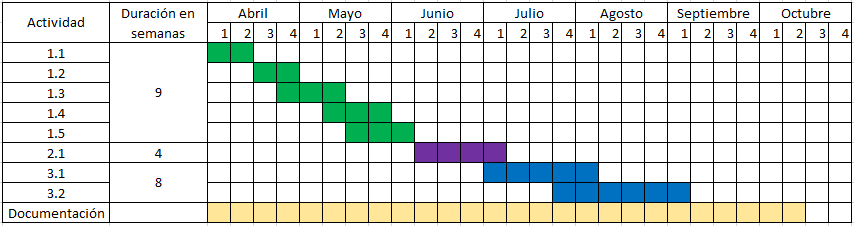
\includegraphics[width=1\linewidth]{Cronograma.PNG}
\label{Cronograma}
\end{figure}

%%%%%%%%%%%%%%%%%%%%%%%%%%%%%%%%%%%%%%%%%%%%%%%%%%%%%%%%%%%%%%%%%%%%%%%%%%%%%%%%%%%%%%%%%%%%%%
\bibliographystyle{abbrv}
\bibliography{BIBLIO.bib}


\section{Anexos}

Carta de aceptación en el programa de movilidad para el semestre 2020-1.
%%%%%%%%%%%%%%%%%%%%%%%%%%%%%%%%%%%%%%%%%%%%%%%%%%%%%%%%%%%%%%%%%%%%%%%%%%%%%%%%%%%%%%%%%%%%%%

%%%%%%%%%%%%%%%%%%%%%%%%%%%%%%%%%%%%%%%%%%%%%%%%%%%%%%%%%%%%%%%%%%%%%%%%%%%%%%%%%%%%%%%%%%%%%%
\end{document}
